\documentclass[border=4pt]{standalone}
\usepackage{pgfplots}
\pgfplotsset{compat=1.18}

\begin{document}
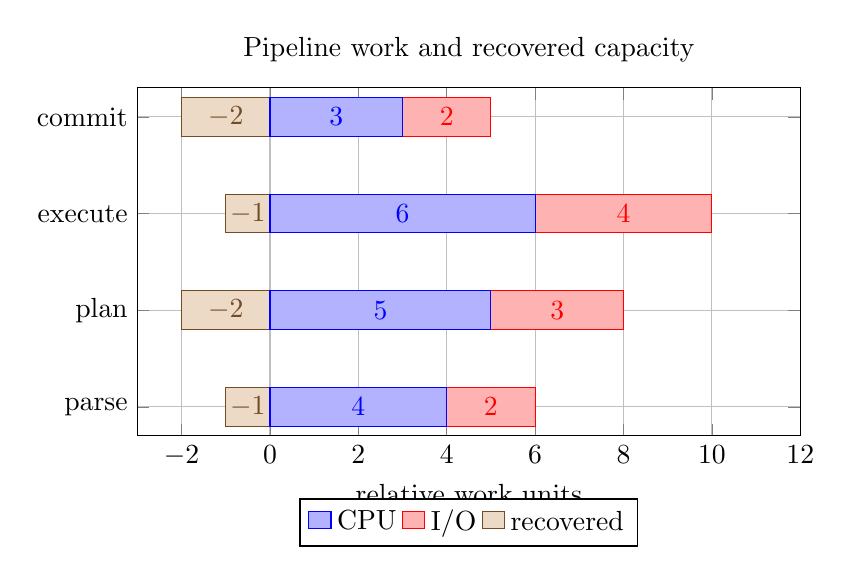
\begin{tikzpicture}
  \begin{axis}[
    xbar stacked,
    width=10cm,
    height=6cm,
    bar width=14pt,
    xmin=-3,
    xmax=12,
    ytick={1,2,3,4},
    yticklabels={parse,plan,execute,commit},
    xlabel={relative work units},
    title={Pipeline work and recovered capacity},
    grid=major,
    nodes near coords,
    legend style={at={(0.5,-0.18)},anchor=north,legend columns=-1}
  ]
    \addplot coordinates {(4,1) (5,2) (6,3) (3,4)};
    \addplot coordinates {(2,1) (3,2) (4,3) (2,4)};
    \addplot coordinates {(-1,1) (-2,2) (-1,3) (-2,4)};
    \legend{CPU,I/O,recovered}
  \end{axis}
\end{tikzpicture}
\end{document}
